 
% \subsection{Streams}
 
% \subsection{Lambda}
 
\subsection{Serialisierung (Nebenläufigkeit und Parallelität)}
% 1 Java ist auch eine Insel - Einführung, Ausbildung, Praxis ; von: Christian Ullenboom
Wenn in Java über Nebenläufigkeit gesprochen wird, sind dabei Threads gemeint. Diese sorgen für eine gleichzeitige Abarbeitung von Programmen bzw. der Ressourcen. Dies kann umgesetzt werden, indem die Hardware mehrere Prozessoren oder Kerne besitzt und diese parallel Prozesse abarbeiten können.
 
Bei einem modernen Ein-Prozessor-Betriebssystem wirkt es oft, als wären die Prozesse parallel, doch dies wird einem nur vorgespielt, indem der Prozessor alle paar Sekunden auf einen anderen Prozess wechselt. Bei einem Betriebssystem mit mehreren Kernen, werden die Prozesse wirklich parallel bearbeitet.
 
\subsubsection{Nebenläufigkeit von Programmen steigert Geschwindigkeit}
Wie nebenläufige Abarbeitung die Performance bei einem Einprozessorsystem beschleunigt, kann an folgendem Beispiel-Programm betrachtet werden:
 
\begin{compactitem}
    \item Programm führt eine Reihe von Befehlen aus
    \item Programm soll Datenbank-Report erstellen/visualisieren    
    \item Dabei können einige Prozesse nebenläufig abgearbeitet werden
    \item Diese Prozesse sind zum Beispiel: Öffnen der Datenbank, Lesen neuer Datensätze gleichzeitig mit dem Analysieren alter Daten, alte Daten können in eine Report-Datei geschrieben werden während neue Daten analysiert werden
    \item Wenn diese Prozesse parallel ausgeführt werden, kann sehr viel Zeit eingespart werden beziehungsweise die Performance sehr erhöht werden.
    \item Dieses Beispiel zeigt allerdings auch, dass Nebenläufigkeit sehr gut geplant werden muss.
\end{compactitem}
 
 
\subsection{Concurrency/Gleichzeitigkeit}
% 0 https://www.baeldung.com/java-util-concurrent
% 0 https://reader.elsevier.com/reader/sd/pii/S0167642305000663?token=33C353917B1806AF8A5D40D069D18442FDCF27727ADE08478255219D5D7D6849BA4E8FAE2A474A3FDCD3CC0A36740643&originRegion=eu-west-1&originCreation=20230105151331
% 1 Java ist auch eine Insel - Einführung, Ausbildung, Praxis; von: Christian Ullenboom
Die Ausführung des Programmcodes wird bei einem modernen Betriebssystem von Prozessen, welche jeweils mindestens einen Thread beherbergen, ausgeführt. Das Interessante daran ist, dass nicht etwa die Prozesse nebenläufig ausgeführt werden, sondern die Threads. Dabei können die Threads auf den gleichen Adressraum zugreifen.
 
\subsubsection{Zustände eines Threads}
\begin{compactitem}
    \item Noch nicht erzeugt: Lebenslauf beginnt mit Schlüsselwort \texttt{new}
    \item Running (Laufend) und Not Running (Nicht laufend); Thread kommt in den Zustand Running, wenn die Methode \texttt{run()} aufgerufen wird. Wenn ein anderer Thread den Prozessor des aktuellen Threads übernimmt, kommt der Thread in den Zustand Not Running.    
    \item Waiting (Wartend): Thread befindet sich in einem Wartezustand
    \item Beendet: Aktivität des Threads wurde beendet
\end{compactitem}
 
\subsection{Aufbau eines Threads}
\subsubsection{Interface Runnable}
Dem Thread muss ein Befehlsobjekt des Typs Runnable übergeben werden \ref{lst:impl:javaRunnable}, um wissen zu können, welcher Code ausgeführt werden soll.
Wenn der Thread gestartet wird, werden die Codezeilen im Befehlsobjekt nebenläufig zum anderen Code in dem Programm ab.
 
\begin{lstlisting}[language=java,caption=Java Runnable,label=lst:impl:javaRunnable]
    interface java.lang.Runnable
\end{lstlisting}
 
Durch dieses Interface kann nun die run()-Methode verwendet werden. \ref{lst:impl:threadExample}
 
\begin{lstlisting}[language=java,caption=Einfaches Thread Beispiel,label=lst:impl:threadExample]
    public class CommandThread implements Runnable { 
        @Override public void run() {   
            ...
            }
        }
\end{lstlisting}
 
Dieser Thread kann nun in einer anderen Klasse verwendet werden, indem er zum Beispiel gestartet (\texttt{thread.start()}) oder gestoppt (\texttt{thread.stop()}) wird. \ref{lst:impl:threadStart}
 
\begin{lstlisting}[language=java,caption=Thread erstellen/starten,label=lst:impl:threadStart]
    Thread t1 = new Thread( new CommandThread() );
    t1.start();
\end{lstlisting}
 
Zusätzlich ist es auch noch möglich, den Thread mit (\texttt{thread.sleep(ms)}) zu pausieren.
 
\subsection{BlockingQueue}
% 1 https://jenkov.com/tutorials/java-util-concurrent/blockingqueue.html#java-blockingqueue-tutorial-video
% 0 https://dl.acm.org/doi/pdf/10.1145/3472456.3472458
% 0 blocking queue:  https://books.google.at/books?id=mvzgNSmHEUAC&pg=PT856&dq=java+blocking+queue&hl=de&sa=X&ved=2ahUKEwiF4Jej3bD8AhUNxwIHHcjWBlMQ6AF6BAgEEAI#v=onepage&q=java%20blocking%20queue&f=false
 
Eine BlockingQueue hat typischerweise einen Thread, welcher Objekte produziert und einen anderen, welcher die Objekte konsumiert. \ref{fig:impl:BlockingQueue}
 
\begin{figure}[h t]
    \centering
    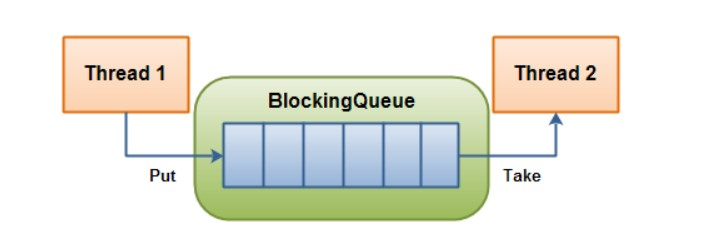
\includegraphics[scale=0.5]{pics/blockingQueue.jpg}
    \caption{Blocking Queue}
    \label{fig:impl:BlockingQueue}
\end{figure}
 
Der produzierende Thread wird weiterhin Objekte produzieren und sie zur BlockingQueue hinzufügen, bis das Limit der Queue erreicht wird. Wenn dieses Limit erreicht wird, wird der Producer-Thread blockiert, während er versucht ein neues Objekt hinzuzufügen. Der Producer Thread bleibt dabei blockiert, bis ein Consumer Thread ein Objekt aus der Queue nimmt.
 
Auf der anderen Seite nimmt der Consumer Thread Objekte aus der Queue, um sie weiter zu verarbeiten. Wenn der Thread versucht ein Objekt aus einer leeren Queue zu nehmen, wird er blockiert, bis der Producer-Thread ein Objekt in die Queue hinzufügt.
 
\subsubsection{BlockingQueue Methoden}
Um die Blocking Queue mit Daten zu bespielen, gibt es spezielle Methoden.
 
\begin{center}
    \begin{tabular}{ |c|c| }
     \hline
     put(o) & fügt Objekte in die BlockingQueue hinzu \\
     \hline
     take() & nimmt Objekte aus der BlockingQueue \\
     \hline
    \end{tabular}
    \end{center}
 
Wenn die Operation bei einer der Methoden erfolglos war, blockiert die Methode, bis die Operation erfolgreich war.
 
\subsubsection{Java Blocking Queue Beispiel}
Das Beispiel unten angeführt verwendet eine ArrayBlockingQueue als Implementation.
 
 
 
\begin{lstlisting}[language=java,caption=Java BlockingQueue Beispiel,label=lst:impl:blockingQueue]
    public class BlockingQueueClass {
    public static void main(String[] args) throws Exception {
        BlockingQueue blockingQueue = new ArrayBlockingQueue(2048);
        Producer producer = new Producer(queue);
        Consumer consumer = new Consumer(queue);
        new Thread(producer).start();
        new Thread(consumer).start();
        Thread.sleep(4000);
    }
    #################################################
 
    public class Producer implements Runnable{
        protected BlockingQueue queue = null;
        public Producer(BlockingQueue queue) {
            this.queue = queue;
        }
        public void run() {
            try {
                queue.put("object1");
                Thread.sleep(1000);
                queue.put("2");
            } catch (InterruptedException e) { e.printStackTrace();}
    }}
    #################################################
    public class Consumer implements Runnable{
        protected BlockingQueue queue = null;
        public Consumer(BlockingQueue queue) {
            this.queue = queue;
        }
        public void run() {
            try {
                System.out.println(queue.take());
                System.out.println(queue.take());
            } catch (InterruptedException e) { e.printStackTrace();}
    }}
}
\end{lstlisting}
 
\subsection{Service executer}
% 0 https://www.baeldung.com/java-executor-service-tutorial
% 1 Java ist auch eine Insel - Einführung, Ausbildung, Praxis; von: Christian Ullenboom
Der Service Executer hilft dabei, den eigentlichen arbeitenden Thread von dem Runnable zu trennen. Denn, wenn ein Thread erzeugt wird, muss das Runnable-Objekt im Konstruktor übergeben werden, dies kann zu Problemen führen, da das Thread-Objekt somit nicht vorher erstellt bzw. aufgebaut werden kann. Ein weiterer Grund, das Runnable und den Thread zu teilen, ist, dass ein Thread nicht einfach so ein anderes Runnable bearbeiten kann, da dieses vorher schon zugewiesen wurde.
 
% \subsection{Java Futures}
% 0 https://www.baeldung.com/java-future
% \subsection{Java Completablefutures}
 
 
% \subsection{First come first serve (Möglichkeiten Prozesse abzuarbeiten)}
 
